\newpage
\subsection*{\textbf{Stability}}

We evaluate the stability of SVEA under 6 common data augmentations; results are shown in Figure \ref{fig:dmc-augs}. SVEA is relatively unaffected by the \textbf{choice of data augmentation} and improves sample efficiency in $\mathbf{27}$ out of $\mathbf{30}$ instances. We further ablate each component of SVEA in Figure \ref{fig:dmc-conv}; we find that both components are key to SVEA's success. We observe that SVEA improves stability in all 27 instances where DrQ is impaired by data augmentation. 
\begin{figure}[H]
    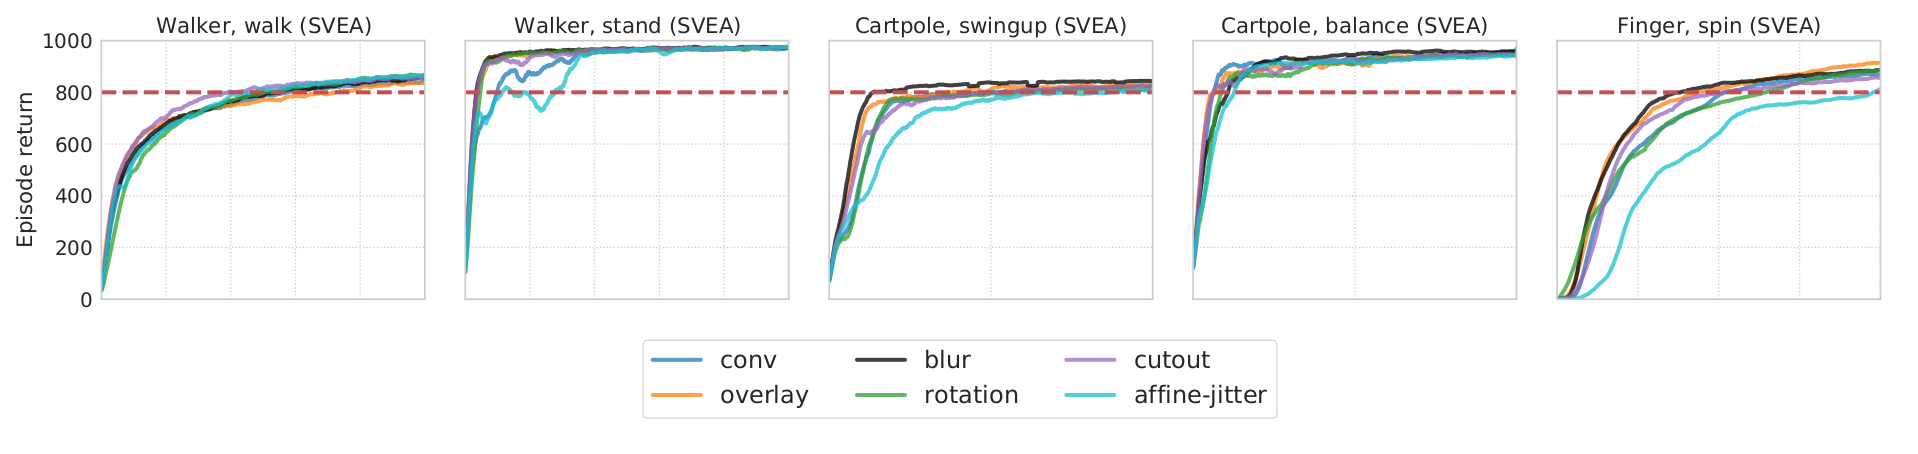
\includegraphics[width=\textwidth]{figures/drq_augs.png}
    \vspace{-0.2in}
    \caption{\textbf{Data augmentations.} Training performance of SVEA under 6 common data augmentations. Mean of 5 seeds. Red line at $800$ return is for visual guidance only. We omit visualization of std. deviations for clarity, but provide per-augmentation comparisons to DrQ (including std. deviations) across all tasks in Figure \ref{fig:drq-augs-suppl}, and test performances in Figure \ref{fig:data-aug-visualization}.}
    \label{fig:dmc-augs}
    \vspace{-0.125in}
\end{figure}
\begin{figure}[H]
    \centering
    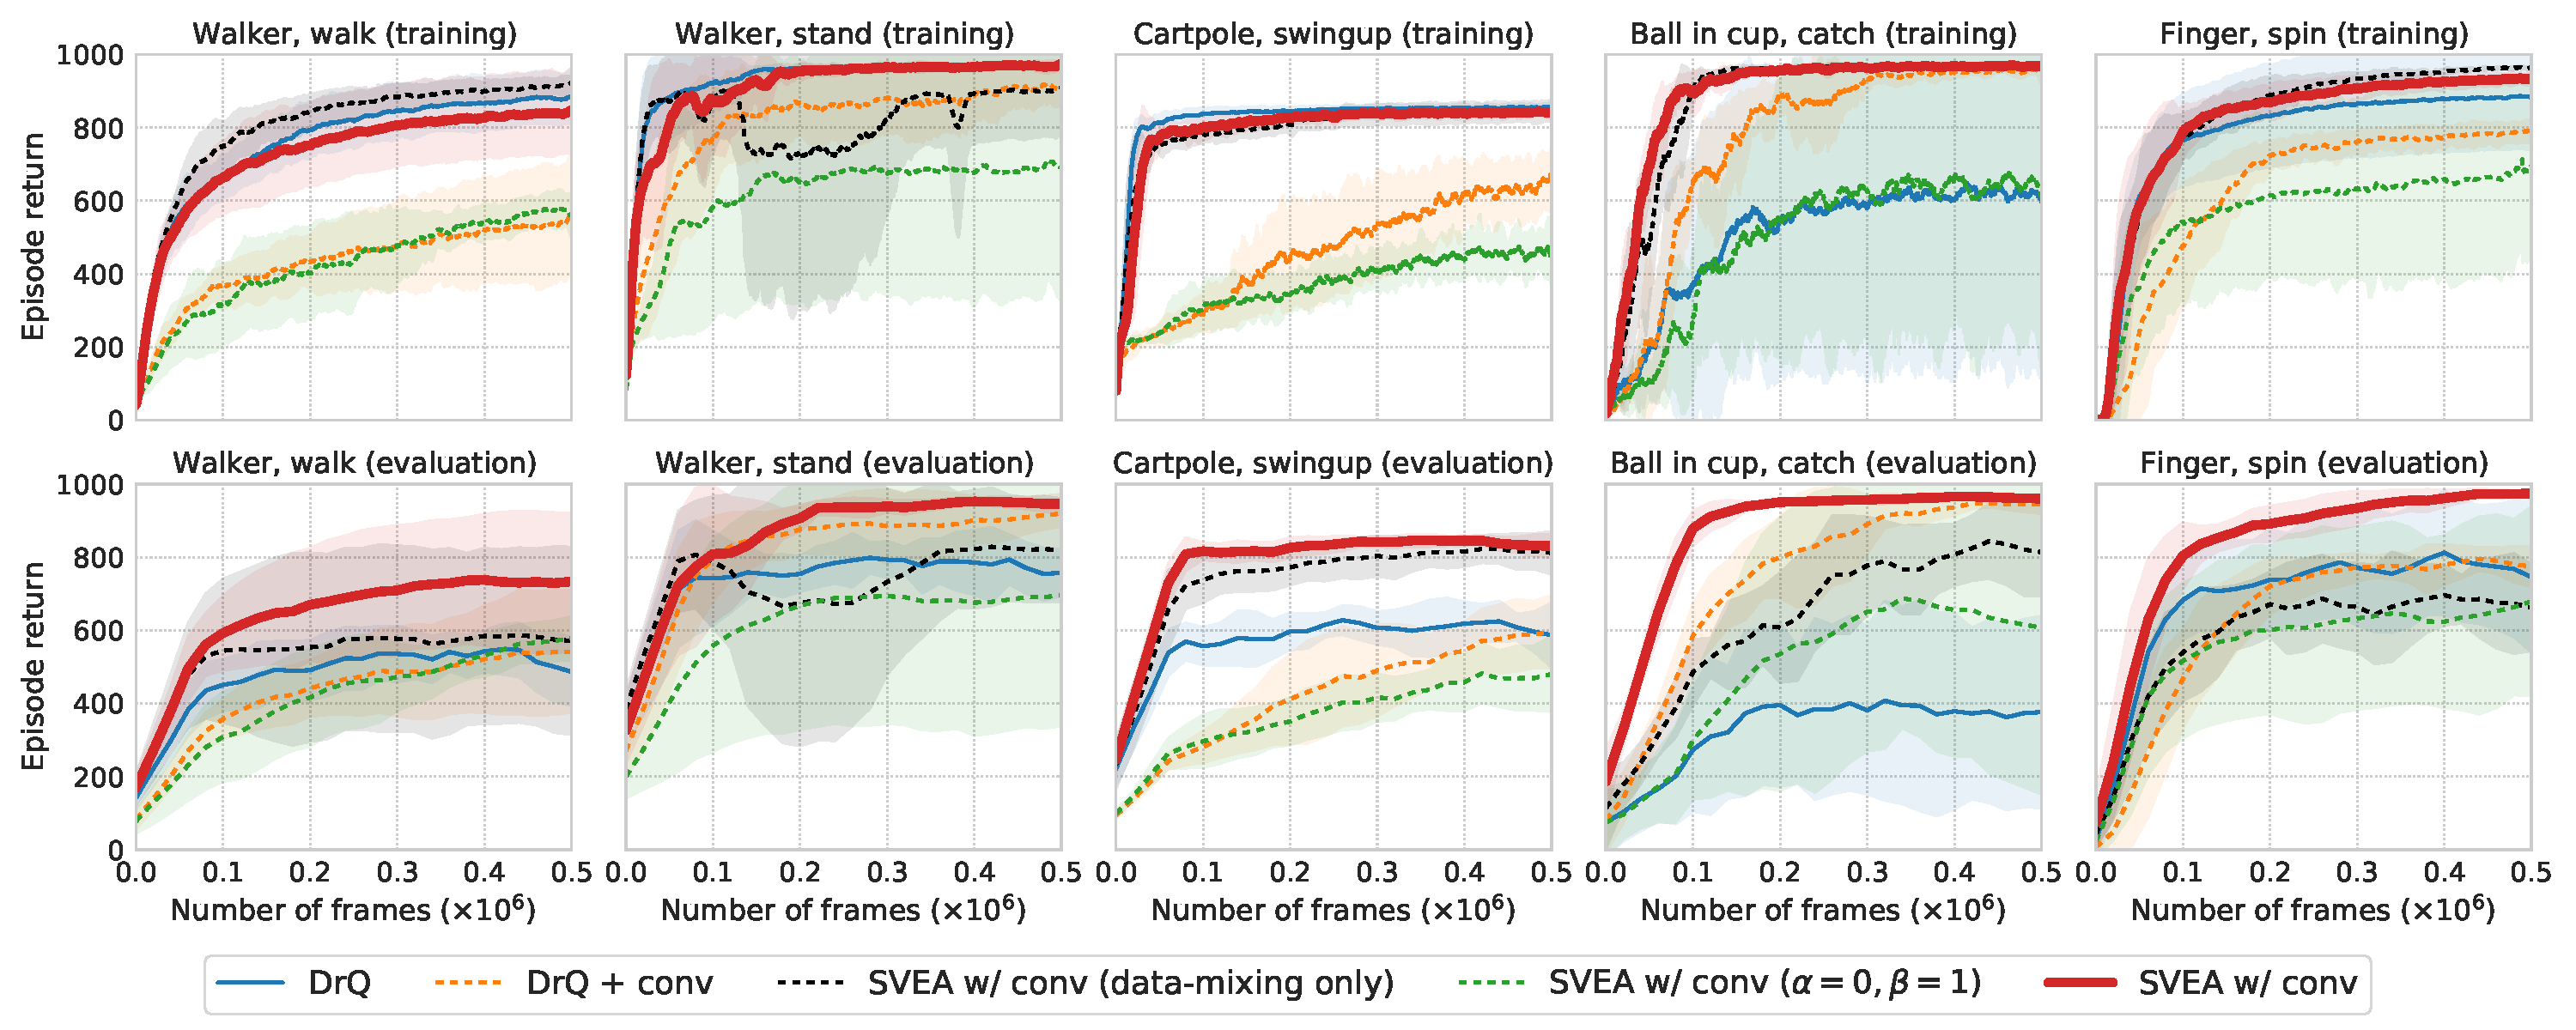
\includegraphics[width=\textwidth]{figures/drq_conv.pdf}
    \vspace{-0.2in}
    \caption{\textbf{Training and test performance.} We compare SVEA to DrQ with and without random convolution augmentation, as well as a set of ablations. \textit{Data-mixing only} indiscriminately applies our data-mixing strategy to all data streams, and $(\alpha=0, \beta=1)$ only augments $Q$-predictions but without data-mixing. We find both components to contribute to SVEA's success. \textit{Top:} episode return on the training environment during training. \textit{Bottom:} generalization measured by episode return on the \texttt{color\_hard} benchmark of DMControl-GB. Mean of 5 seeds, shaded area is $\pm1$ std. deviation.}
    \label{fig:dmc-conv}
    \vspace{-0.125in}
\end{figure}\\

\subsubsection*{\textbf{Stability under data augmentation}}
\label{sec:stability-under-data-augmentation}

Figure \ref{fig:drq-augs-suppl} compares the sample efficiency and stability of SVEA and DrQ under each of the 6 considered data augmentations for 5 tasks from DMControl. Stability of DrQ under data augmentation is found to be highly sensitive to both the choice of augmentation and the particular task. For example, the \textit{DrQ + aug} baseline is relatively unaffected by a majority of data augmentations in the \textit{Walker}, \textit{stand} task, while we observe significant instability across all data augmentations in the \textit{Cartpole}, \textit{swingup} task. Our results therefore indicate that SVEA can be a highly effective method for eliminating the need for costly trial-and-error associated with application of data augmentation.
\begin{figure}[H]
    \centering
    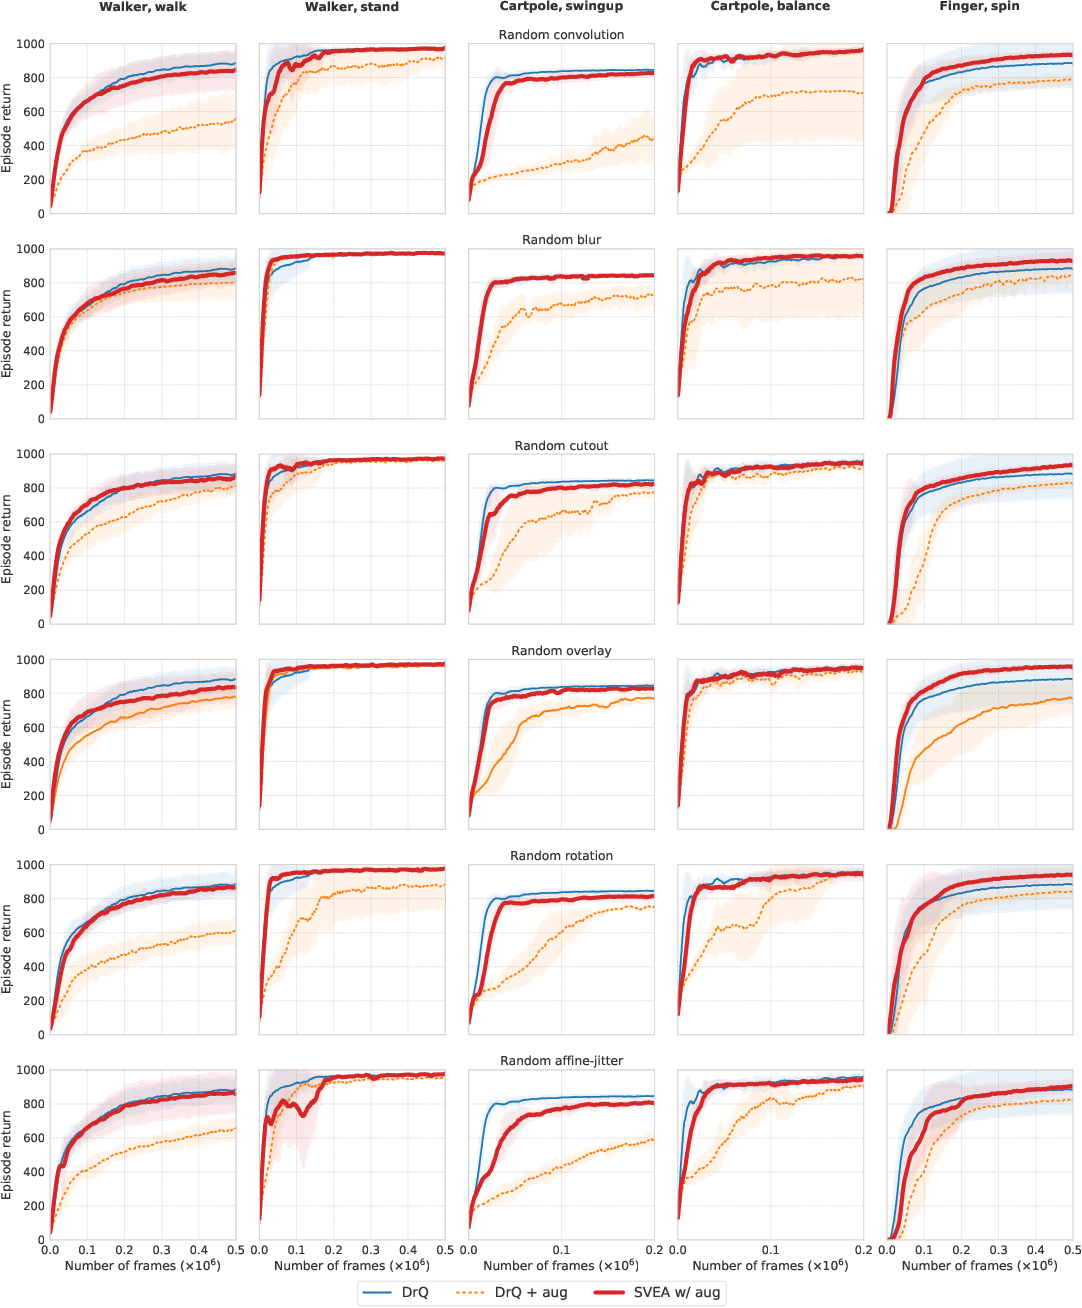
\includegraphics[width=\textwidth]{figures/drq_augs_suppl.png}
    \caption{\textbf{Stability under data augmentation.} Training performance measured by episode return of SVEA and DrQ under 6 common data augmentations (using ConvNets). We additionally provide reference curves for DrQ without additional augmentation. Mean of 5 seeds, shaded area is $\pm1$ std. deviation. SVEA obtains similar sample efficiency to DrQ without augmentation, while the sample efficiency of \textit{DrQ + aug} is highly dependent on the task and choice of augmentation.}
    \label{fig:drq-augs-suppl}
    \vspace{-0.1in}
\end{figure}